
\section{Introduction}
\label{introduction}


%\textcolor[rgb]{1.00,0.00,0.00}{We need to put a brief introduction to the case study right here.}

The Power Level Angle (PLA) signal processing system is part of the Full Authority Digital Engine Control System (FADEC), 
 which provides engine control during flight to achieve stable and transient engine characteristics. 
 In the engine control system, the PLA signal processing system is not only a typical system instance of continuous quantity processing, but also the pivotal section assisting pilots controlling the aircraft through the power levers.
 For PLA signal processing system, we emphasize on the following questions: 1) whether the input signal is correctly processed by the system for one period. 2) whether the system can keep the output correct for a long period of time. 3) whether each part of the system can respond a sudden exception of input in real time.
 In this paper, we are going to use a simplified PLA signal processing system of real application as a case study. 
 
 The purpose of PLA signal processing system is to convert the obtained throttle stick signal value into the original throttle stick angle value and judge it. 
 If it is judged that there is no fault, then it will return the corresponding value of the PLA signal after processing and set a fault signal to invalid, 
 representing that the system has no PLA signal fault in current period. 
 Otherwise it will return the fault information and set the fault signal to valid.

Fig.1 shows the system structure of our case. There are two diagnosis modules, a sensor data unit and a data conversion unit. The sensor data unit task is connected to the BIT diagnosis unit and the data conversion unit direactly while the latter two units are connected to the Extremum \& Slope diagnosis unit. BIT diagnosis module consists of three diagnosis units and a decider unit and, analogously, the Extremum \& Slope diagnosis module consists of two diagnosis units and a decider unit. Besides BIT diagnosis module, the calibration conversion unit is also driven by sensor data unit task and provides signal for Extremum \& Slope diagnosis module.

\begin{figure}[ht!]
	\centering
	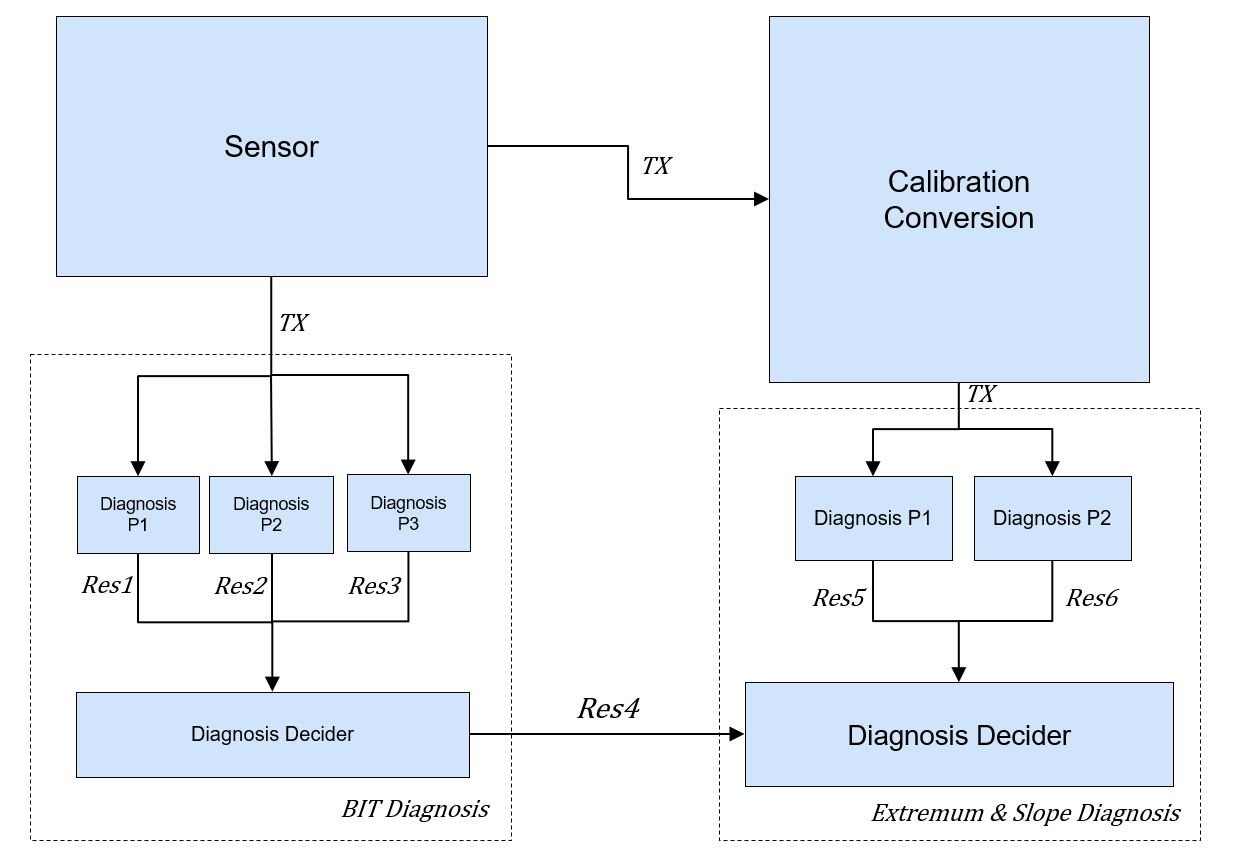
\includegraphics[width=90mm]{figure/sys_structure.jpg}
	\caption{The system structure}
	\label{sys_structure}
\end{figure}

In order to verificate the PLA signal processing system, we use the BIP framework. To help validating the system, we apply NuXmv tool chain on the NuXmv system model which is transformed from the BIP model. In this case, we have to write a series of properties in CTL or LTL specification patterns. To avoid mistake on transforming requirements to specifications and fully specify the PLA signal processing system, we sort out the requirements and write monitors adding to the BIP model. Fig.2 shows the work flow according to our two different system designs.

\begin{figure}[ht!]
	\centering
	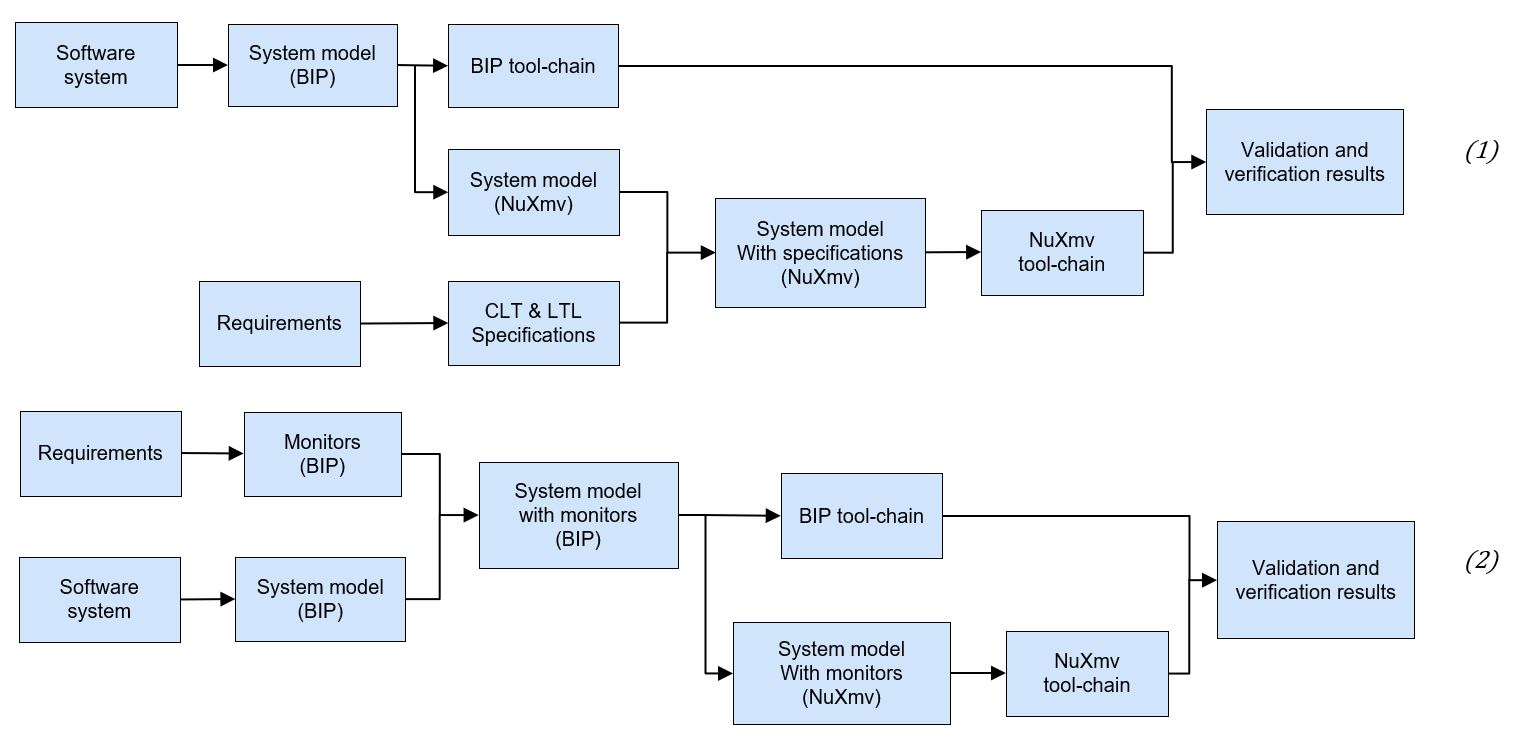
\includegraphics[width=110mm]{figure/work_flow.jpg}
	\caption{(1) Work flow of system model with specification 
		     \protect\\(2) Work flow of system model with monitors}
	\label{work_flow}
\end{figure}

%There are three modules in the system. PLA signals will first undergo a BIT Diagnosis module, 
% then be calibrated and converted into physical quantities. 
% After the Extremum and Slope Diagnosis module, it will finally generate the PLA fault signal for output.
%
%The Built-int Test(BIT) refers to the detection and monitoring of the system and its own equipment. 
% In the PLA signal processing system model, the BIT Diagnosis realizes the analog quantity, 
% or periodic fault detection of circuits such as fault location and processing based on the diagnosis results.
%
%The calibration conversion module's function is to collect the signal from signal collector. 
% The arriving signal will be converted to the corresponding engineering value by means of a calibration curve or an index table.
%
%An Extremum/Slope Diagnosis module contains extremum diagnosis and slope diagnosis.
% The function of extremum diagnosis is to judge whether the current signal is in valid range since the PLA signal processing system cannot handle illegal data. 
% The function of slope diagnosis is to give the constraint of the magnitude of the change between the two adjacent signals.
%
%The three modules introduced above work together for giving a credible output signal. 
%
%
%The BIP (Behavior, Interaction, Priority) framework is a component-based system design framework \cite{bip11}.
% It advocates the rigorous system design methodology \cite{sifakis13}, 
% which has been proposed as a response to the grand challenge of complex hardware/software mixed system design \cite{sifakis2015}.
% The concept of rigorous system design can be understood as a formal, accountable and coherent process 
% for deriving correct-by-construct system implementations from high-level specifications.
% The essential safety properties of the design are guaranteed at the earliest possible design phase by applying algorithmic verification to the system model,
% and then the system implementation is automatically generated by a sequence of property preserving model transformations,
% progressively refining the model with details specific to the target platforms.
%
%The BIP framework provides a well defined modeling language and an associated toolbox to realize the rigorous system design flow.
% The modeling language allows the construction of composite components from atomic components through layered application of interactions and of priorities.
% The BIP toolbox supports both verification of high-level system designs ~\cite{dfinder10,atva15,tgc15}
% and automatic model transformation and code generation of low-level implementations from high-level system designs~\cite{bip-emsoft10}.
% In practice, BIP has been actively used in several applications~\cite{bipapplication12a,bipapplication18}.
% 
 
%We achieve requirement modeling and validation in two steps.
% First,  requirements of the system are analysed and formalised. In this step, we need to decompose the system into functional modules.
% Then, atomic components realising the basic functionality of the system are designed (components previously designed for other systems can be reused).
% Finally, the resulting system is checked for deadlock-freedom.
% Properties, which are not enforced by construction through architecture application, must be verified a posteriori.
% In this case study, we illustrate all steps of this process, except the requirement formalisation.


% It provides a simple, but powerful mechanism for the coordination of concurrent components by superposing three layers.
% First, component behaviour is described by Labelled Transition Systems (LTS) having transitions labelled with ports.
% Ports form the interface of a component and are used to define its interactions with other components.
% Second, interaction models, i.e. sets of interactions, define the component coordination.
% Interactions are sets of ports that define allowed synchronizations between components.
% An interaction model is defined in a structured manner by using connectors.
% Third, priorities are used to impose scheduling constraints and to resolve conflicts when multiple interactions are enabled simultaneously.


%Design, manufacture and verification of large scale reliable hardware/software systems 
% (e.g. cyber-physical systems) remains a grand challenge in system design automation~\cite{sifakis2015}.
% To address this challenge, the rigorous system design methodology~\cite{sifakis13}.


The rest of the paper is structured as follows.
%
In Section~\ref{sec:preliminary} and Section~\ref{sec:bip}, we introduce the preliminaries and the BIP modeling language.
%
In Section~\ref{sec:relatework} and Section~\ref{sec:conclusions}, we review the most related works and draw some conclusions and outline directions for future work.

